\documentclass{beamer}
\mode<presentation>
\usepackage{amsmath,amssymb,mathtools}
\usepackage{textcomp}
\usepackage{gensymb}
\usepackage{adjustbox}
\usepackage{subcaption}
\usepackage{enumitem}
\usepackage{multicol}
\usepackage{listings}
\usepackage{url}
\usepackage{graphicx} % <-- needed for images
\def\UrlBreaks{\do\/\do-}

\usetheme{Boadilla}
\usecolortheme{lily}
\setbeamertemplate{footline}{
  \leavevmode%
  \hbox{%
  \begin{beamercolorbox}[wd=\paperwidth,ht=2ex,dp=1ex,right]{author in head/foot}%
    \insertframenumber{} / \inserttotalframenumber\hspace*{2ex}
  \end{beamercolorbox}}%
  \vskip0pt%
}
\setbeamertemplate{navigation symbols}{}

\lstset{
  frame=single,
  breaklines=true,
  columns=fullflexible,
  basicstyle=\ttfamily\tiny   % tiny font so code fits
}

\numberwithin{equation}{section}

% ---- your macros ----
\providecommand{\nCr}[2]{\,^{#1}C_{#2}}
\providecommand{\nPr}[2]{\,^{#1}P_{#2}}
\providecommand{\mbf}{\mathbf}
\providecommand{\pr}[1]{\ensuremath{\Pr\left(#1\right)}}
\providecommand{\qfunc}[1]{\ensuremath{Q\left(#1\right)}}
\providecommand{\sbrak}[1]{\ensuremath{{}\left[#1\right]}}
\providecommand{\lsbrak}[1]{\ensuremath{{}\left[#1\right.}}
\providecommand{\rsbrak}[1]{\ensuremath{\left.#1\right]}}
\providecommand{\brak}[1]{\ensuremath{\left(#1\right)}}
\providecommand{\lbrak}[1]{\ensuremath{\left(#1\right.}}
\providecommand{\rbrak}[1]{\ensuremath{\left.#1\right)}}
\providecommand{\cbrak}[1]{\ensuremath{\left\{#1\right\}}}
\providecommand{\lcbrak}[1]{\ensuremath{\left\{#1\right.}}
\providecommand{\rcbrak}[1]{\ensuremath{\left.#1\right\}}}
\theoremstyle{remark}
\newtheorem{rem}{Remark}
\newcommand{\sgn}{\mathop{\mathrm{sgn}}}
\providecommand{\abs}[1]{\left\vert#1\right\vert}
\providecommand{\res}[1]{\Res\displaylimits_{#1}}
\providecommand{\norm}[1]{\lVert#1\rVert}
\providecommand{\mtx}[1]{\mathbf{#1}}
\providecommand{\mean}[1]{E\left[ #1 \right]}
\providecommand{\fourier}{\overset{\mathcal{F}}{ \rightleftharpoons}}
\providecommand{\system}{\overset{\mathcal{H}}{ \longleftrightarrow}}
\providecommand{\dec}[2]{\ensuremath{\overset{#1}{\underset{#2}{\gtrless}}}}
\newcommand{\myvec}[1]{\ensuremath{\begin{pmatrix}#1\end{pmatrix}}}
\let\vec\mathbf

\title{Matgeo Presentation - Problem 4.13.67}
\author{ee25btech11063 - Vejith}

\begin{document}


\frame{\titlepage}
\begin{frame}{Question}
The area of the triangle formed by the intersection of line parallel to X axis and passing through $\Vec{p}$(h,k) with the lines y=x and x+y=2 is 4h$^2$.Find the locus of point $\Vec{p}$
\end{frame}

\begin{frame}{Solution}
line parallel to X axis is of the form 
\begin{align}
    \Vec{n}^T\Vec{x}=c.\\
     \implies \brak{0\hspace{0.5cm}1}\myvec{x\\y}=c.
\end{align}
As the above line passes through $\Vec{p}$(h,k)
\begin{align}
     \brak{0\hspace{0.5cm}1}\myvec{h\\k}=c.
     \implies c=k.
\end{align}
The three lines are as follows
\begin{align}
    y=k\implies \brak{0\hspace{0.5cm}1}\myvec{x\\y}=k.\\
    -x+y=0 \implies \brak{-1\hspace{0.5cm}1}\myvec{x\\y}=0.
    \end{align}
    \begin{align}
    x+y=2 \implies\brak{1\hspace{0.5cm}1}\myvec{x\\y}=2.
\end{align}
    \end{frame}

    \begin{frame}{Solution}
Let $\Vec{A}$,$\Vec{B}$,$\Vec{C}$ be the point of intersection of above 3 lines\\
On solving equation (0.4) and (0.5)
\begin{align}
    \begin{pmatrix}
        0 & 1\\
        -1 & 1
    \end{pmatrix} \myvec{x\\y}=\myvec{k\\0}.\\
    \implies \vec{A}=\myvec{x\\y}=\myvec{k\\k}
\end{align}
On solving equation (0.5) and (0.6)
\begin{align}
    \begin{pmatrix}
        -1 & 1\\
        1 & 1
    \end{pmatrix} \myvec{x\\y}=\myvec{0\\2} &\xrightarrow{R_2 \leftrightarrow R_1+R_2} \begin{pmatrix}
        -1 & 1\\
        0 & 2
    \end{pmatrix} \myvec{x\\y}=\myvec{0\\2}.\\
 \implies \vec{B}=\myvec{x\\y}=\myvec{1\\1}
\end{align}
On solving equation (0.4) and (0.6)
\begin{align}
    \begin{pmatrix}
        0 & 1\\
        1 & 1
    \end{pmatrix} \myvec{x\\y}=\myvec{k\\2}.
    \end{align}
    \end{frame}

    \begin{frame}{Solution}
        \begin{align}
    \implies \vec{C}=\myvec{x\\y}=\myvec{2-k\\k}
\end{align}
\begin{align}
    \text{area of }\triangle \text{ABc}=\frac{1}{2}\norm{(\vec{A}-\vec{B})\times(\vec{B}-\vec{C})}\\
    =\frac{1}{2}\norm{\myvec{k-1\\k-1}\times\myvec{k-1\\1-k}}\\
    =\frac{1}{2}(2(k-1)^2)=(k-1)^2.
\end{align}
Given area of the triangle formed by the intersection of above 3 lines is 4h$^2$.
\begin{align}
    \implies (k-1)^2= 4h^2.\\
    \implies (y-1)^2=4x^2\\
    \implies(y-1-2x)(y-1+2x)=0
    \end{align}
    \end{frame}

    \begin{frame}{Conclusion}
        $\implies$ The locus of $\vec{p}$ is Pair of  straight lines
    \begin{align}
     y-1-2x=0. \implies  \brak{-2\hspace{0.5cm}1}\myvec{x\\y}=1.\\
     y-1+2x=0. \implies  \brak{2\hspace{0.5cm}1}\myvec{x\\y}=1.
   \end{align}
    \end{frame}
    
    

\begin{frame}{Plot}
    \begin{figure}[H]
    \centering
    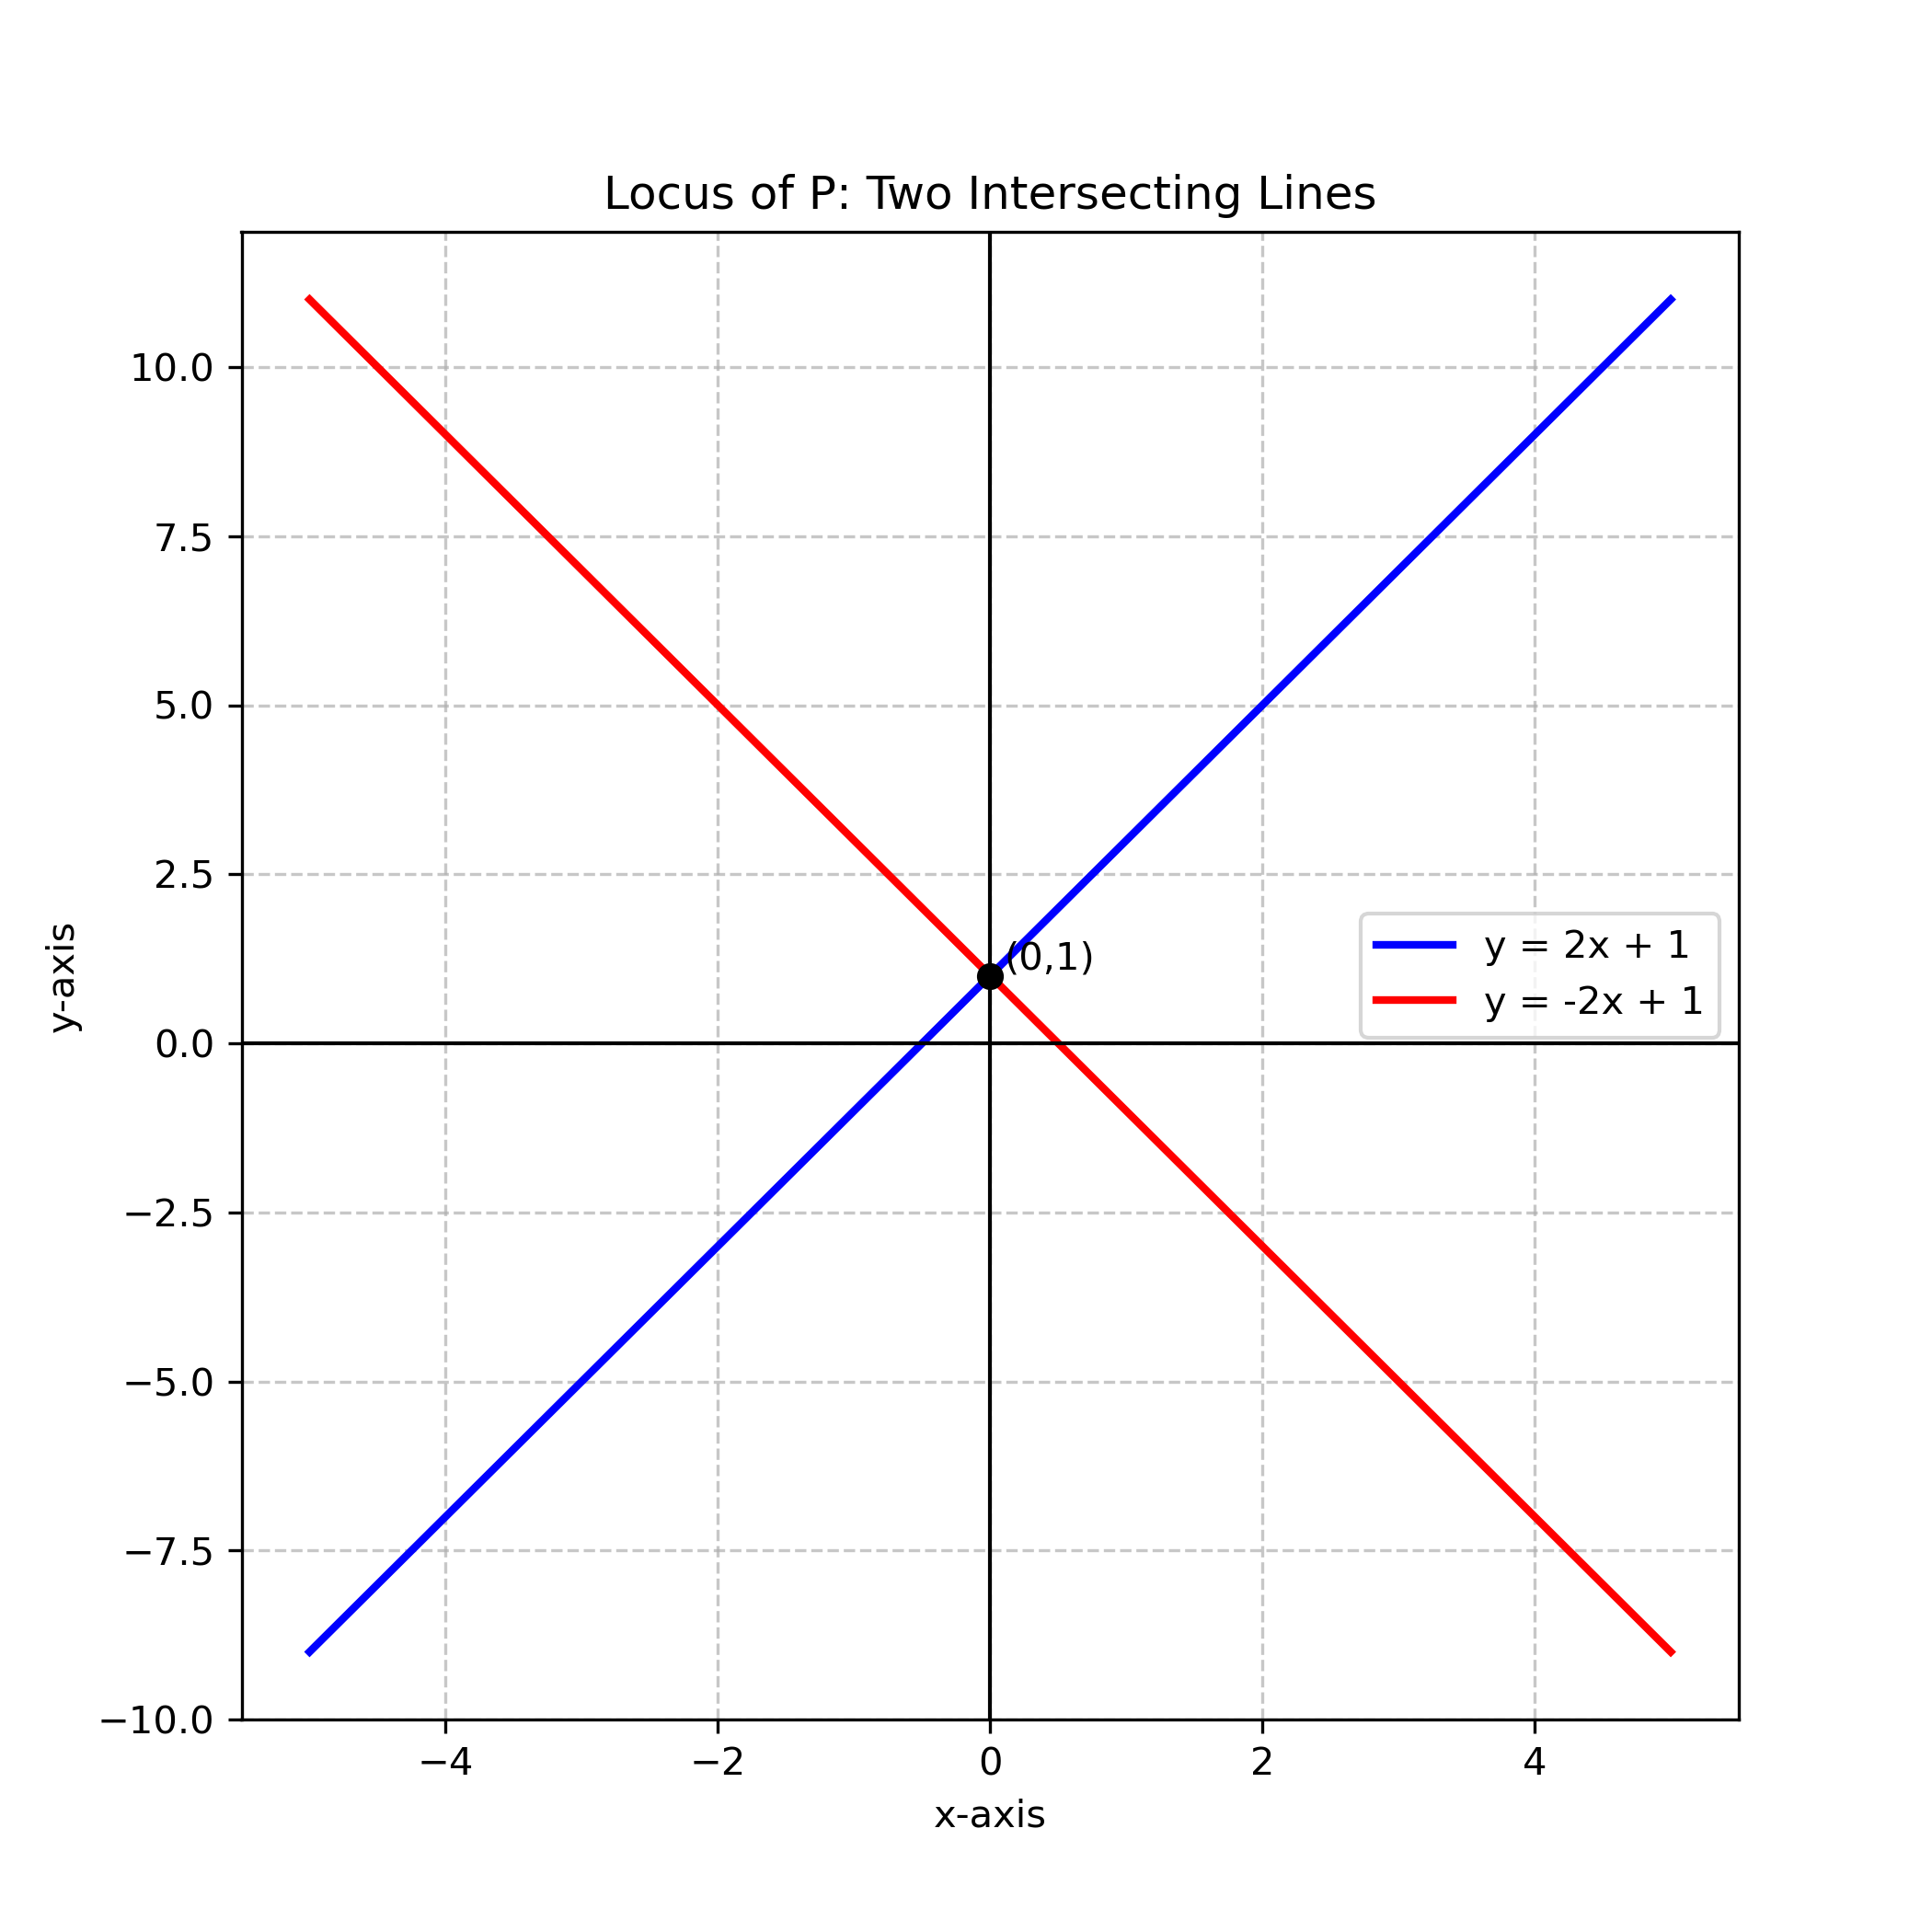
\includegraphics[width=0.70\columnwidth]{figs/01.png}
    \label{fig-1}
\end{figure}
\end{frame}

% --------- CODE APPENDIX ---------
\section*{Appendix: Code}

% C program
\begin{frame}[fragile]{C Code: locus.c}
\begin{lstlisting}[language=C]
#include <stdio.h>

int main() {
    FILE *fp;

    // Open the file locus.dat in write mode
    fp = fopen("locus.dat", "w");

    if (fp == NULL) {
        printf("Error opening file!\n");
        return 1;
    }

    // Write the solution into the file
    fprintf(fp, "The locus of P is given by the equation:\n");
    fprintf(fp, "(y - 1)^2 = 4x^2\n");
    fprintf(fp, "Which represents two intersecting straight lines:\n");
    fprintf(fp, "1) y - 1 = 2x  -->  y = 2x + 1\n");
    fprintf(fp, "2) y - 1 = -2x -->  y = -2x + 1\n");

    // Close the file
    fclose(fp);

    printf("Locus has been written successfully into locus.dat\n");

    return 0;
}
\end{lstlisting}
\end{frame}

\begin{frame}[fragile]{Python: plot.py}
\begin{lstlisting}[language=Python]
 import numpy as np
import matplotlib.pyplot as plt

# Define range for x
x = np.linspace(-5, 5, 400)

# Equations of the two lines
y1 = 2*x + 1
y2 = -2*x + 1

# Create the plot
plt.figure(figsize=(7, 7))

# Plot both lines
plt.plot(x, y1, label="y = 2x + 1", color="blue", linewidth=2)
plt.plot(x, y2, label="y = -2x + 1", color="red", linewidth=2)

# Mark the point of intersection (0,1)
plt.scatter(0, 1, color="black", zorder=5)
plt.text(0.1, 1.1, "(0,1)", fontsize=10)

# Axes setup
plt.axhline(0, color="black", linewidth=1)
plt.axvline(0, color="black", linewidth=1)

# Labels, grid and title
plt.xlabel("x-axis")
plt.ylabel("y-axis")
plt.title("Locus of P: Two Intersecting Lines")
plt.grid(True, linestyle="--", alpha=0.7)
plt.legend()
plt.savefig("locus_plot.png", dpi=300)
plt.show()

\end{lstlisting}
\end{frame} 
\end{document}
